\documentclass[12pt,preprintnumbers,amsmath,amssymb,nofootinbib,superscriptaddress]{revtex4-1}
\usepackage[paperheight=12cm,top=0.5cm,bottom=0.5cm,left=1cm,right=1cm]{geometry}
\usepackage{xparse}
\NewDocumentCommand{\DIV}{om}{%
  \IfValueT{#1}{\setcounter{#2}{\numexpr#1-1\relax}}%
  \csname #2\endcsname
}

\usepackage[latin1]{inputenc}
\usepackage{slashed}
\usepackage{amsmath}
\usepackage{textcomp}
\usepackage{amssymb}
\usepackage{amsfonts}
\usepackage{indentfirst}
\usepackage{color}
\usepackage[dvipsnames]{xcolor}
\usepackage{hyperref}
\usepackage{subcaption}
\usepackage{graphicx,graphics}
\graphicspath{{figures/}}
\usepackage[skins,theorems,many]{tcolorbox}
\tcbset{highlight math style={enhanced,
  colframe=red,colback=white,arc=0pt,boxrule=1pt}}
\usepackage[abs]{overpic}
\usepackage{xcolor,varwidth}
\usepackage[english]{babel}
\usepackage{blindtext,tikz}
\usetikzlibrary{calc}
\usepackage{fancyhdr}
\usepackage{tikz}
\usetikzlibrary{positioning}
\usepackage{algorithm}
\usepackage{algorithmic}
\usepackage{algorithmicx}
\usepackage{algpseudocode}
\def\bibsection{\section*{}} %Removes black line above refrences

%--------------------------%
%----- COLOURED BOXES -----%
%--------------------------%

%Blue equation box
%\tcbhighmath[colframe=RoyalBlue!70!black,colback=RoyalBlue!25!white]{

%Orange equation box
%\tcbhighmath[colframe=BurntOrange!95!black,colback=BurntOrange!45!white]{

%Purple equation box
%\tcbhighmath[colframe=Purple!150!black,colback=Purple!30!white]{

%Green equation box
%\tcbhighmath[colframe=ForestGreen,colback=ForestGreen!25!white]{

%Grey equation box
%\tcbhighmath[colframe=Black,colback=Black!10!white]{

%Pink equation box
%\tcbhighmath[colframe=magenta,colback=magenta!20!white]{

%Blue and red equation box
%\tcbhighmath[frame style={left color=RoyalBlue!70!black,right color=Red!95!black},interior style={left color=RoyalBlue!35!white,right color=Red!50!white}]{

%Red and green equation box
%\tcbhighmath[frame style={left color=Red!95!black,right color=ForestGreen},interior style={left color=Red!50!white,right color=ForestGreen!25!white}]{

\begin{document}

\tikz[overlay,remember picture] % ArXiv number
{
    \node at ($(current page.west)+(1,0)$) [rotate=90] {\Large\textcolor{gray}{}};
}

\pagenumbering{gobble}

\hfill{16-02-2023} % Conference name and date

\vspace{2.5cm}

\title{
\tcbhighmath[frame style={left color=RoyalBlue!70!black,right color=Red!95!black},interior style={left color=RoyalBlue!35!white,right color=Red!50!white},boxrule=2pt]{
\text{\Large Algoritma \& Struktur Data}
}}

\author{Kristina P. Sinaga}

%\affiliation{Theoretical Particle Physics and Cosmology, King's College London, WC2R 2LS, UK}


\maketitle

\newpage

%-----EXAMPLE SLIDES-----%

\newpage

\DIV[1]{section}{HEADLINE}\label{Ueff}
\vspace{-0.7cm}
\DIV[1]{subsection}{Summary}
\vspace{-0.2cm}\hrule

\vspace{2cm}

\begin{enumerate}
    \item Membahas definisi algoritma sebagai sekumpulan instruksi yang memecahkan masalah tertentu atau melakukan tugas tertentu. 
    \item Pentingnya struktur data dalam mengatur dan mengelola data dalam algoritma.
    \item Penggunaan Pseudocode untuk mendeskripsikan algoritma dengan cara yang terstruktur.
\end{enumerate}

\vspace{1cm}

\newpage


\DIV[1]{section}{Section 1}\label{Ueff}
\vspace{-0.7cm}
\DIV[1]{subsection}{Konsep Dasar Struktur Data}
\vspace{-0.2cm}\hrule

\vspace{2cm}

\begin{enumerate}
    \item Algoritma dan struktur data adalah dua konsep dasar dalam ilmu komputer yang terkait erat dan memainkan peran penting dalam menyelesaikan masalah komputasi secara efisien.
    \item Untuk merancang algoritme yang efisien, penting untuk memiliki pemahaman yang baik tentang struktur data yang tersedia dan propertinya, dan untuk memilih struktur data yang paling tepat untuk tugas yang sedang dikerjakan. 
    \item Untuk merancang struktur data yang efektif, penting untuk mempertimbangkan jenis operasi yang akan dilakukan pada data dan memilih struktur yang akan mengoptimalkan operasi tersebut.
\end{enumerate}

\vspace{1cm}

\newpage

\DIV[1]{section}{Section 1}\label{Ueff}
\vspace{-0.7cm}
\DIV[2]{subsection}{Defenisi Algoritma}
\vspace{-0.2cm}\hrule

\vspace{2cm}

\begin{enumerate}
    \item Algoritma adalah seperangkat instruksi langkah demi langkah yang dirancang untuk memecahkan masalah tertentu atau menyelesaikan tugas tertentu. 
    \item Dalam ilmu komputer, algoritma biasanya diimplementasikan sebagai program atau fungsi yang mengambil data masukan dan menghasilkan data keluaran. 
    \item Algoritma dapat dianalisis berdasarkan kompleksitas waktu dan kompleksitas ruangnya, yang masing-masing mengacu pada jumlah waktu dan sumber daya memori yang diperlukan untuk menjalankan algoritme.
\end{enumerate}

\vspace{1cm}

\newpage

\DIV[1]{section}{Section 1}\label{Ueff}
\vspace{-0.7cm}
\DIV[2]{subsection}{Contoh Algoritma}
\vspace{-0.2cm}\hrule

\vspace{2cm}
Beberapa contoh algoritma:
\begin{enumerate}
    \item Algoritma pengurutan \textit{(sorting)}: Algoritma pengurutan digunakan untuk mengatur daftar item dalam urutan tertentu, seperti urutan naik atau turun. Contoh algoritma pengurutan termasuk pengurutan gelembung, pengurutan penyisipan, pengurutan pilihan, pengurutan gabungan, dan pengurutan cepat.
    \item Algoritme pencarian: Algoritme pencarian digunakan untuk menemukan item tertentu dalam daftar item. Contoh algoritma pencarian termasuk pencarian linier dan pencarian biner.
    \item Algoritme pembelajaran mesin \textit{(Machine learning)}: Algoritma pembelajaran mesin digunakan untuk mempelajari pola dan hubungan dalam data, dan dapat digunakan untuk tugas-tugas seperti klasifikasi, regresi, dan pengelompokan. Contoh algoritma pembelajaran mesin termasuk regresi linier, regresi logistik, k-nearest neighbor (KNN), pohon keputusan, dan jaringan syaraf tiruan (ANN).
\end{enumerate}

\vspace{1cm}

\newpage

\DIV[1]{section}{Section 1}\label{Ueff}
\vspace{-0.7cm}
\DIV[3]{subsection}{Defenisi Struktur Data}
\vspace{-0.2cm}\hrule

\vspace{2cm}

\begin{enumerate}
    \item Struktur data, di sisi lain, adalah cara mengatur dan menyimpan data dalam program komputer. Struktur data menyediakan cara untuk merepresentasikan dan memanipulasi data, dan struktur data yang berbeda dioptimalkan untuk operasi yang berbeda. 
    \item Contoh umum dari struktur data meliputi larik, daftar tertaut, tumpukan, antrean, pohon, dan grafik.
\end{enumerate}

\vspace{1cm}

\newpage

\DIV[1]{section}{Section 1}\label{Ueff}
\vspace{-0.7cm}
\DIV[4]{subsection}{Contoh Struktur Data}
\vspace{-0.2cm}\hrule

\vspace{2cm}
Berikut adalah beberapa contoh umum dari struktur data:
\begin{enumerate}
    \item Array: Array adalah kumpulan elemen, masing-masing diidentifikasi dengan indeks atau kunci. Array digunakan untuk menyimpan kumpulan elemen sekuensial berukuran tetap dari tipe yang sama, seperti daftar angka.
    \item Daftar tertaut \textit{(linked lists)}: Daftar tertaut adalah kumpulan elemen, masing-masing berisi nilai dan referensi ke elemen berikutnya dalam daftar. Daftar tertaut dapat digunakan untuk menyimpan kumpulan elemen yang dipesan dengan berbagai ukuran dan jenis, dan sering digunakan untuk mengimplementasikan tumpukan dan antrean.
\end{enumerate}

\vspace{1cm}

\newpage

\DIV[1]{section}{Section 1}\label{Ueff}
\vspace{-0.7cm}
\DIV[4]{subsection}{Contoh Struktur Data}
\vspace{-0.2cm}\hrule

\vspace{2cm}
Berikut adalah beberapa contoh umum dari struktur data:
\begin{enumerate}
    \item Antrian: Antrian adalah kumpulan elemen yang mendukung dua operasi: enqueue, yang menambahkan elemen ke belakang antrean, dan dequeue, yang menghapus elemen depan dari antrean. Antrian sering digunakan dalam aplikasi yang memerlukan perilaku first-in-first-out (FIFO), seperti penjadwalan pekerjaan di sistem operasi.
    \item Pohon: Pohon adalah struktur data hierarkis yang terdiri dari simpul-simpul yang memiliki hubungan induk-anak. Pohon sering digunakan untuk merepresentasikan hubungan hierarkis, seperti struktur sistem file atau organisasi situs web.
\end{enumerate}

\vspace{1cm}

\newpage

\DIV[1]{section}{Section 1}\label{Ueff}
\vspace{-0.7cm}
\DIV[4]{subsection}{Contoh Struktur Data}
\vspace{-0.2cm}\hrule

\vspace{2cm}
Berikut adalah beberapa contoh umum dari struktur data:
\begin{enumerate}
    \item Tumpukan: Tumpukan adalah kumpulan elemen yang mendukung dua operasi: push, yang menambahkan elemen ke bagian atas tumpukan, dan pop, yang menghapus elemen teratas dari tumpukan. Tumpukan sering digunakan dalam aplikasi yang memerlukan perilaku last-in-first-out (LIFO), seperti fungsi undo/redo di editor teks.
    \item Tabel hash: Tabel hash adalah struktur data yang memetakan kunci ke nilai menggunakan fungsi hash. Tabel hash sering digunakan untuk pencarian cepat dan digunakan di banyak aplikasi, seperti pengindeksan database dan caching.
\end{enumerate}

\vspace{1cm}

\newpage

\DIV[1]{section}{Section 1}\label{Ueff}
\vspace{-0.7cm}
\DIV[5]{subsection}{Contoh Penggunaan Algoritma dan Struktur Data}
\vspace{-0.2cm}\hrule

\vspace{2cm}

\begin{enumerate}
    \item Pemilihan struktur data dapat berdampak signifikan pada efisiensi algoritma yang beroperasi pada data tersebut. Misalnya, beberapa algoritme mungkin memerlukan akses cepat ke masing-masing elemen data, sementara yang lain mungkin memerlukan penyisipan atau penghapusan elemen yang efisien. Pemilihan struktur data juga dapat memengaruhi kompleksitas ruang suatu algoritma, karena struktur data yang berbeda membutuhkan jumlah memori yang berbeda untuk menyimpan data yang sama.
\end{enumerate}

\vspace{1cm}

\newpage

\DIV[1]{section}{Section 1}
\vspace{-0.7cm}
\DIV[6]{subsection}{Subsection B}
\vspace{-0.2cm}
\hrule

\vspace{0.8cm}

\begin{minipage}{0.6\textwidth}
    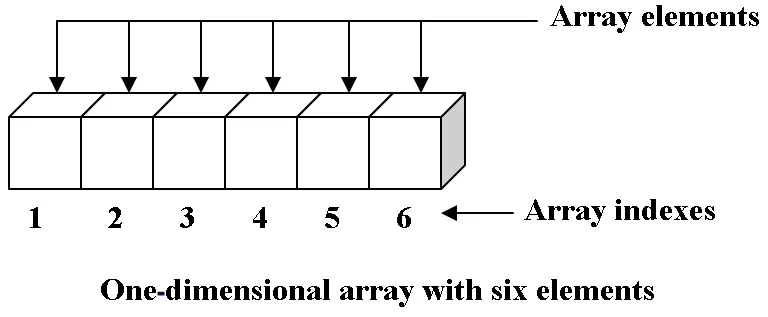
\includegraphics[width=\linewidth]{Figures/array.png}
\vspace{-2cm}

\end{minipage}
\begin{minipage}{0.39\textwidth}

\begin{itemize}
    \item Tipe data abstrak (ADT) adalah cara menentukan sekumpulan operasi yang dapat dilakukan pada tipe data, tanpa menentukan bagaimana operasi tersebut diimplementasikan.
\end{itemize}


\vspace{1cm}

\end{minipage}


\vspace{1cm}

\newpage

\DIV[1]{section}{Section 1}\label{Ueff}
\vspace{-0.7cm}
\DIV[7]{subsection}{Notasi ALgoritma}
\vspace{-0.2cm}\hrule

\vspace{2cm}


\begin{itemize}
    \item Notasi algoritma adalah cara untuk menyatakan kompleksitas waktu dan ruang dari suatu algoritma dengan menggunakan notasi matematika. Notasi yang paling umum digunakan adalah notasi $O$ besar, Omega besar, dan Theta besar.
    \item Notasi $O$ besar, diwakili oleh simbol "$O$", digunakan untuk menggambarkan batas atas kompleksitas waktu atau ruang dari suatu algoritma. Ini mengungkapkan skenario terburuk untuk algoritma, atau jumlah maksimum waktu atau ruang yang dapat digunakan algoritma. Misalnya, jika suatu algoritma memiliki kompleksitas waktu $O(n)$, itu berarti waktu yang dibutuhkan untuk menjalankan algoritma tumbuh secara linier dengan ukuran input.
\end{itemize}


\vspace{1cm}

\newpage

\DIV[1]{section}{Section 1}\label{Ueff}
\vspace{-0.7cm}
\DIV[8]{subsection}{Representasi Grafis dari Sebuah Algoritma}
\vspace{-0.2cm}\hrule

\vspace{2cm}


\begin{itemize}
    \item Representasi grafis umum dari suatu algoritma adalah flowchart. Diagram alir menggunakan simbol dan panah yang berbeda untuk mewakili berbagai langkah dan keputusan yang terlibat dalam pemecahan masalah. Berikut adalah contoh diagram alir untuk algoritme sederhana untuk menemukan maksimum dua angka:
    \item Dalam diagram alir:
    \begin{enumerate}
        \item kotak persegi panjang mewakili langkah-langkah proses
        \item kotak berbentuk wajik mewakili titik keputusan
        \item Panah mewakili alur algoritma
    \end{enumerate} 
\end{itemize}


\vspace{1cm}

\newpage

\DIV[1]{section}{Section 1}\label{Ueff}
\vspace{-0.7cm}
\DIV[8]{subsection}{Mencari Nilai Maximum 2 Bilangan}
\vspace{-0.2cm}\hrule

\vspace{1cm}

\begin{tikzpicture}[node distance=0.5cm]
  % Define the nodes
  \node (start) [rectangle, draw] {Start Algorithm};
  \node (input) [rectangle, draw, below=of start] {Input a, b};
  \node (decision) [diamond, draw, below=of input] {$a > b$};
  \node (set_a) [rectangle, draw, right=of decision, xshift=2cm] {Set max = a};
  \node (set_b) [rectangle, draw, below=of decision, yshift=-0.5cm] {Set max = b};
  \node (output) [rectangle, draw, below=of set_a] {Output max};
  \node (end) [rectangle, draw, below=of output] {End Algorithm};
  % Connect the nodes with arrows
  \draw [->] (start) -- (input);
  \draw [->] (input) -- (decision);
  \draw [->] (decision) -- node[above] {yes} (set_a);
  \draw [->] (decision) -- node[right] {no} (set_b);
  \draw [->] (set_a) -- (output);
  \draw [->] (set_b) -- (output);
  \draw [->] (output) -- (end);
\end{tikzpicture}

\begin{itemize}
    \item Algoritma dimulai dengan input dua angka, a dan b, dan kemudian memeriksa mana yang lebih besar. Jika a lebih besar dari b, maka algoritme menetapkan nilai maksimum ke a. Jika tidak, itu menetapkan nilai maksimum ke b. Akhirnya, algoritme mengeluarkan nilai maksimum dan berakhir.
\end{itemize}


\vspace{1cm}

\newpage


\DIV[1]{section}{Section 1}\label{Ueff}
\vspace{-0.7cm}
\DIV[9]{subsection}{Simbol flowchart}
\vspace{-0.2cm}\hrule

\vspace{2cm}

Berikut adalah beberapa simbol flowchart yang umum digunakan:

\begin{itemize}
    \item Simbol terminal (oval): digunakan untuk menunjukkan awal dan akhir dari flowchart.
    \item Simbol proses (persegi panjang): digunakan untuk mewakili proses atau tindakan yang dilakukan.
    \item Simbol keputusan (diamond): digunakan untuk mewakili titik keputusan atau pertanyaan dengan dua atau lebih kemungkinan jawaban.
    \item Simbol input/output (jajar genjang): digunakan untuk mewakili operasi input atau output.
    \item Simbol konektor (lingkaran): digunakan untuk menghubungkan berbagai bagian diagram alur.
\end{itemize}


\vspace{1cm}

\newpage

\DIV[1]{section}{Section 1}\label{Ueff}
\vspace{-0.7cm}
\DIV[9]{subsection}{Simbol flowchart}
\vspace{-0.2cm}\hrule

\vspace{2cm}

Berikut adalah beberapa simbol flowchart yang umum digunakan:

\begin{itemize}
    \item Simbol konektor (lingkaran): digunakan untuk menghubungkan berbagai bagian diagram alur.
    \item Simbol konektor di luar halaman (dua garis paralel): digunakan untuk menghubungkan bagian-bagian diagram alur yang terletak di halaman atau lembaran berbeda.
    \item Simbol proses yang telah ditentukan sebelumnya (persegi panjang dengan garis ganda di sisinya): digunakan untuk mewakili proses yang sudah ditentukan atau didokumentasikan di tempat lain.
    \item Simbol penundaan (bentuk setengah kapsul): digunakan untuk menunjukkan penundaan atau masa tunggu di diagram alur.
\end{itemize}


\vspace{1cm}

\newpage

\DIV[1]{section}{Section 1}\label{Ueff}
\vspace{-0.7cm}
\DIV[9]{subsection}{Simbol flowchart}
\vspace{-0.2cm}\hrule

\vspace{2cm}

Berikut adalah beberapa simbol flowchart yang umum digunakan:

\begin{itemize}
    \item Simbol dokumen (persegi panjang dengan dasar bergelombang): digunakan untuk menunjukkan suatu dokumen atau laporan dalam flowchart.
    \item Simbol database (silinder): digunakan untuk mewakili database atau lokasi penyimpanan data.
\end{itemize}


\vspace{1cm}

\newpage

\DIV[1]{section}{Section 1}\label{Ueff}
\vspace{-0.7cm}
\DIV[10]{subsection}{Algoritma Pseudocode }
\vspace{-0.2cm}\hrule

\vspace{1cm}

\begin{itemize}
    \item Pseudocode adalah bahasa informal tingkat tinggi yang digunakan untuk menggambarkan logika program komputer. Ini bukan bahasa pemrograman tertentu, melainkan cara untuk merepresentasikan langkah-langkah yang terlibat dalam memecahkan masalah atau mengimplementasikan algoritme menggunakan sintaks mirip bahasa alami.
    \item Pseudocode dapat ditulis dengan cara terstruktur atau tidak terstruktur. 
    \item Pseudocode terstruktur menggunakan struktur kontrol seperti loop, pernyataan bersyarat, dan subrutin untuk menggambarkan logika suatu program.
   \item Pseudocode tidak terstruktur menggunakan pernyataan sederhana seperti bahasa Inggris untuk menggambarkan logika suatu program.
\end{itemize}


\vspace{1cm}

\newpage

\DIV[1]{section}{Section 1}\label{Ueff}
\vspace{-0.7cm}
\DIV[10]{subsection}{Algoritma Pseudocode }
\vspace{-0.2cm}\hrule

\vspace{0.7cm}
\begin{itemize}
    \item Algoritma pseudocode ini menjelaskan proses sederhana untuk menambahkan dua angka bersama dan menampilkan hasilnya.
    \item \begin{algorithmic}[1]
  \State $a \gets 1$
  \If{$a > 0$}
    \State $b \gets 2$
    \If{$b > a$}
      \State $c \gets a + b$
    \Else
      \State $c \gets b - a$
    \EndIf
  \EndIf
  \State \Return $c$
\end{algorithmic}
\end{itemize}


\vspace{1cm}

\DIV[]{section}{KESIMPULAN}\label{Ueff}
\vspace{-0.7cm}
\DIV[]{subsection}{}
\vspace{-0.2cm}\hrule

\vspace{2cm}

\begin{enumerate}
    \item algoritma adalah konsep dasar dalam ilmu komputer dan digunakan untuk memecahkan berbagai macam masalah di berbagai bidang. 
    \item Memahami konsep kunci dan elemen algoritma, seperti struktur data, pseudocode, dan bagan alur \textit{(flowchart)}, dapat membantu dalam pengembangan algoritme yang efisien dan efektif untuk tugas tertentu.
\end{enumerate}

\vspace{1cm}

\vspace{\fill}
\centering
\href{https://kpnaga08.github.io/}{Kristina P. Sinaga}


\end{document}